% adapté de la RIG version française

\documentclass[french]{./sageo}

\confShortName{SAGEO'2017}
\confLongName{SAGEO'2017 - Rouen, 6-9 novembre 2017}

\usepackage[utf8]{inputenc} 
\usepackage[T1]{fontenc}
\usepackage{lmodern}
\usepackage{textcomp}
\usepackage{amsmath}
\usepackage{graphicx}
\usepackage{multirow}
\usepackage[noend]{algorithmic}
\usepackage[linesnumbered,ruled,vlined,boxed,commentsnumbered]{algorithm2e}

%% user packages and macros

\usepackage{ragged2e}





\firstpagenumber{1}


\title[Causalités Spatio-temporelles]{Une méthode d'identification de causalités dans des données spatio-temporelles}

\author[1,2]{Juste}{Raimbault}


% addresses are automatically numbered
\address{UMR CNRS 8504 Géographie-cités}
        {}
\address{UMR-T 9403 IFSTTAR LVMT}
        {juste.raimbault@polytechnique.edu}       

\resume{Résumé.}


\motscles{Quelques mots clés}

\keywords{En anglais}

\abstract{Abstract in English}

\begin{document}

\maketitle

\newpage



%%%%%%%%%%%%%%%
\section{Introduction}
%%%%%%%%%%%%%%%



L'étude des processus spatio-temporels fortement couplés implique la prise en compte d'intrications entre ceux-ci généralement difficiles à isoler. Essence même des approches par la complexité, ces interactions qui sont à l'origine du comportement émergent d'un système font sens comme objet d'étude en lui-même, et une séparation des processus paraît alors contradictoire avec une vision intégrée du système. Dans le cas des systèmes territoriaux, l'exemple des interactions entre réseaux de transport et territoires est une excellente allégorie de ce phénomène : des méthodes isolant les ``effets structurants'' d'une infrastructure développées dans les années 70~\cite{bonnafous1974methodologies} se sont révélées par la suite de l'instrumentation politique et sans fondement empirique~\cite{offner1993effets}. Le débat est toujours d'actualité puisque la question se pose toujours par exemple pour la construction de lignes à grande vitesse~\cite{crozethalshs01094554}. La réalité des processus territoriaux est en fait bien plus compliqué qu'une simple relation causale entre la mise en place d'une infrastructure et les retombées sur le développement local, mais correspond bien d'une \emph{co-évolution} complexe~\cite{bretagnolletel00459720}. Sur le temps long et à grande échelle, certains effets de renforcement des dynamiques dans les systèmes de villes par l'insertion dans les réseaux, ont été mis en valeur par l'application de la Théorie Evolutive des Villes~\cite{espacegeo2014effets}, montrant que le démêlage est toutefois possible dans certains cas par une compréhension plus globale du système. A une autre échelle, toujours concernant les relations entre réseaux et territoires, on peut citer les liens entre pratiques de mobilité, étalement urbain et localisation des ressources dans un cadre métropolitain~\cite{cerqueira2017inegalites} qui s'avèrent tout autant complexes. Ce type de problématique est bien sûr présent dans d'autres domaines : en Economie Géographique, l'exemple des liens entre innovation, impacts locaux de la connaissance et aggregation des agents économiques est une illustration typiques de processus économiques spatio-temporels présentant des causalités circulaires difficiles à démêler~\cite{audretsch1996r}. Des méthodes spécifiques sont introduites, comme l'utilisation d'instruments statistiques comme par~\cite{aghion2015innovation} dans lequel l'origine géographique des membres du Bureau du Congrès américain attribuant les subventions locales est une bonne variable instrumentale pour lier caractère innovant et inégalités des plus haut salaire, et permet de montrer que la correlation significative entre les deux est en fait une causalité de l'innovation sur les inégalités.


Le couplage fort spatio-temporel implique généralement l'introduction de la notion de causalité, à laquelle la géographie s'est toujours intéressée : \cite{loi1985etude} montre que les questions fondamentales que se pose la géographie théorique récente (isolation des objects, lien entre espace et structures causales, etc.) étaient déjà présentes dans la géographie classique de Vidal. \cite{claval1985causalite} critique d'ailleurs les nouveaux déterminismes ayant émergé, notamment celui proposé par certains tenants de l'analyse systémique. François Durand-Dastès a plus récemment répondu indirectement à ces critiques dans \cite{durand2003geographes}


Les régimes sous lesquels des identifications de causalité sont cohérentes ne sont pas identifiés de manière évidente. Ceux-ci dépendront des définition utilisées, de la même manière que les méthodes à disposition pour lesquelles nous pouvons donner quelques illustrations. \cite{liu2011discovering} propose la detection de relations spatio-temporelles entre perturbations des flots de trafic, introduisant une définition particulière de la causalité basé sur une correspondance de points extrêmes. Les algorithmes associés sont toutefois spécifiques et difficilement applicables à des types de systèmes différents. Les neurosciences ont développé de nombreuses méthodes répondant à des problématiques similaires. \cite{luo2013spatio} définit une causalité de Granger généralisée prenant en compte la non-stationnarité et s'appliquant à des régions abstraites issues d'imagerie fonctionnelle.



%%%%%%%%%%%%%%%
\section{Méthode}
%%%%%%%%%%%%%%%


Nous décrivons ici une méthode générique, basée sur un test similaire à la causalité de Granger~\cite{}, pour tenter d'identifier des relations causales dans des systèmes spatiaux. Soit $X_j(\vec{x},t)$ des processus aléatoires spatiaux unidimensionnels. Une réalisation d'un sous-système territorial est donnée par des ensembles de trajectoires pour chaque processus $x_{i,j,t}$. On suppose l'existence de fonctions de correspondance $\Phi_{j1,j2}$ permettant de faire correspondre les réalisations de chaque composantes à un index unique (dans le cas le plus simple, on associera les variables sur les mêmes patches). Si $\textrm{argmax}_{\tau} \hat{\rho}\left[x_{j_1},x_{j_2}\right]$ est clairement défini % TODO notion trop floue ? le problème est que des modèles stat conditionnent trop ?
, son signe donnera alors le sens de la causalité entre les composantes $j_1$ et $j_2$.


% TODO some kind of smoothing has to be introduced, either as preprocessing or as part of the optimization process (at least for first observed behavior on synthetic data. maybe it is typical of the model ?)
% - formalize mean estimator on repetitions, compare it to a direct estimator (// computation or aggregated data ?)







%%%%%%%%%%%%%%%
\section{Résultats}
%%%%%%%%%%%%%%%


%%%%%%%%%%%%%%%
\subsection{Données Synthétiques}

Cette méthode doit dans un premier temps être testée et partiellement validée, ce que nous proposons de faire sur des données synthétiques. % TODO cit Rochebrune ?
En écho à l'exemple des relations entre réseaux de transport et territoires qui a permis d'introduire notre problématique précédemment, nous proposons de générer des configurations urbaines stylisées dans lesquelles réseau et densité s'influencent mutuellement, et pour lesquelles les causalités ne sont pas évidents \emph{a priori} étant donné les paramètres du modèle génératif.\cite{raimbault2014hybrid} décrit et explore un modèle simple de morphogenèse urbaine (modèle RBD) répondant parfaitement à ces contraintes. En effet, les variables explicatives de la croissance urbaine, les processus d'extension du réseau et le couplage entre densité urbaine et réseau sont assez élémentaires. Cependant, hormis dans des cas extrêmes (distance au centre détermine valeur foncière uniquement, le réseau dépendra de manière causale de la densité, ou distance au réseau seule, la causalité devrait être inversée), les régimes mixtes n'exhibent pas de causalités évidentes : c'est donc un parfait cas pour tester si la méthode est capable d'en détecter.

Nous utilisons une implémentation adaptée\footnote{disponible sur le dépôt ouvert du projet à\\\texttt{https://github.com/JusteRaimbault/CityNetwork/tree/master/Models/Simple/ModelCA}} du modèle initial, permettant de capturer les valeurs des variables étudiées pour chaque patch et à chaque pas de temps et de calculer les correlations retardées entre variables au sein du modèle.

Nous explorons une grille de l'espace des paramètres du modèle RDB, faisant varier les paramètres de poids de la densité, de la distance au centre et de la distance au réseau, que l'on note respectivement $(w_{d},w_{c},w_{r})$, dans $\left[0;1\right]$ avec un pas de 0.1. Les autres paramètres sont fixés à leur valeurs par défaut données dans l'article. Pour chaque valeur des paramètres, nous procédons à $N=100$ répétitions ce qui est suffisant pour une bonne convergence des indicateurs. Les explorations sont effectuées via le logiciel OpenMole~\cite{reuillon2013openmole}.

Nous calculons sur l'ensemble des patches les corrélations retardées entre les variables suivantes : densité locale, distance au centre et distance au réseau. Des regroupements par régimes peuvent se faire, lorsqu'un paramètre domine et impose le régime




%%%%%%%%%%%%%%%
\begin{figure*}[h]
\centering
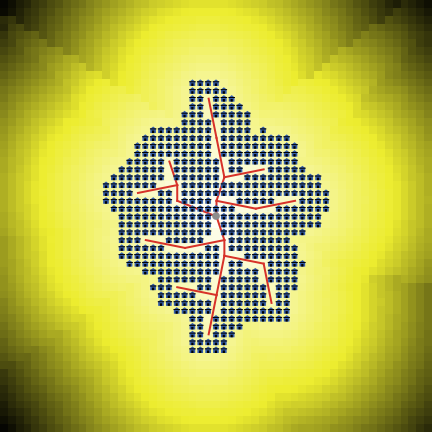
\includegraphics[width=3.9cm]{figures/ex_60_wdens0_wroad1_wcenter1_seed272727}
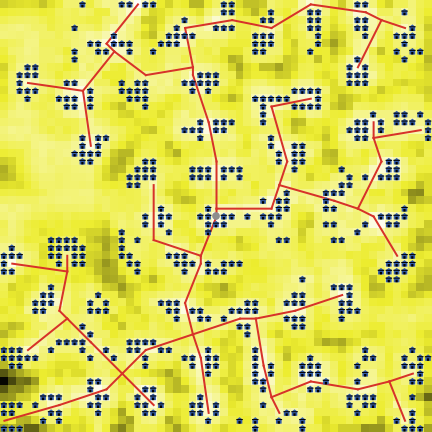
\includegraphics[width=3.9cm]{figures/ex_60_wdens1_wroad1_wcenter0_seed272727}
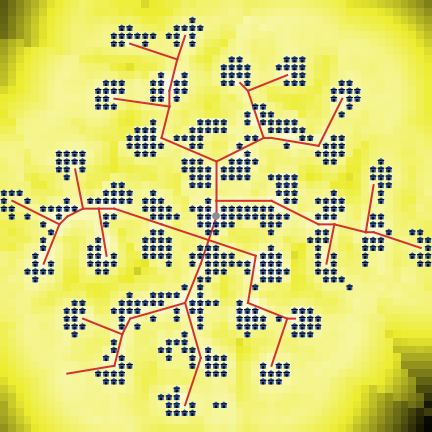
\includegraphics[width=3.9cm]{figures/ex_60_wdens1_wroad1_wcenter1_seed272727}\\\vspace{0.2cm}
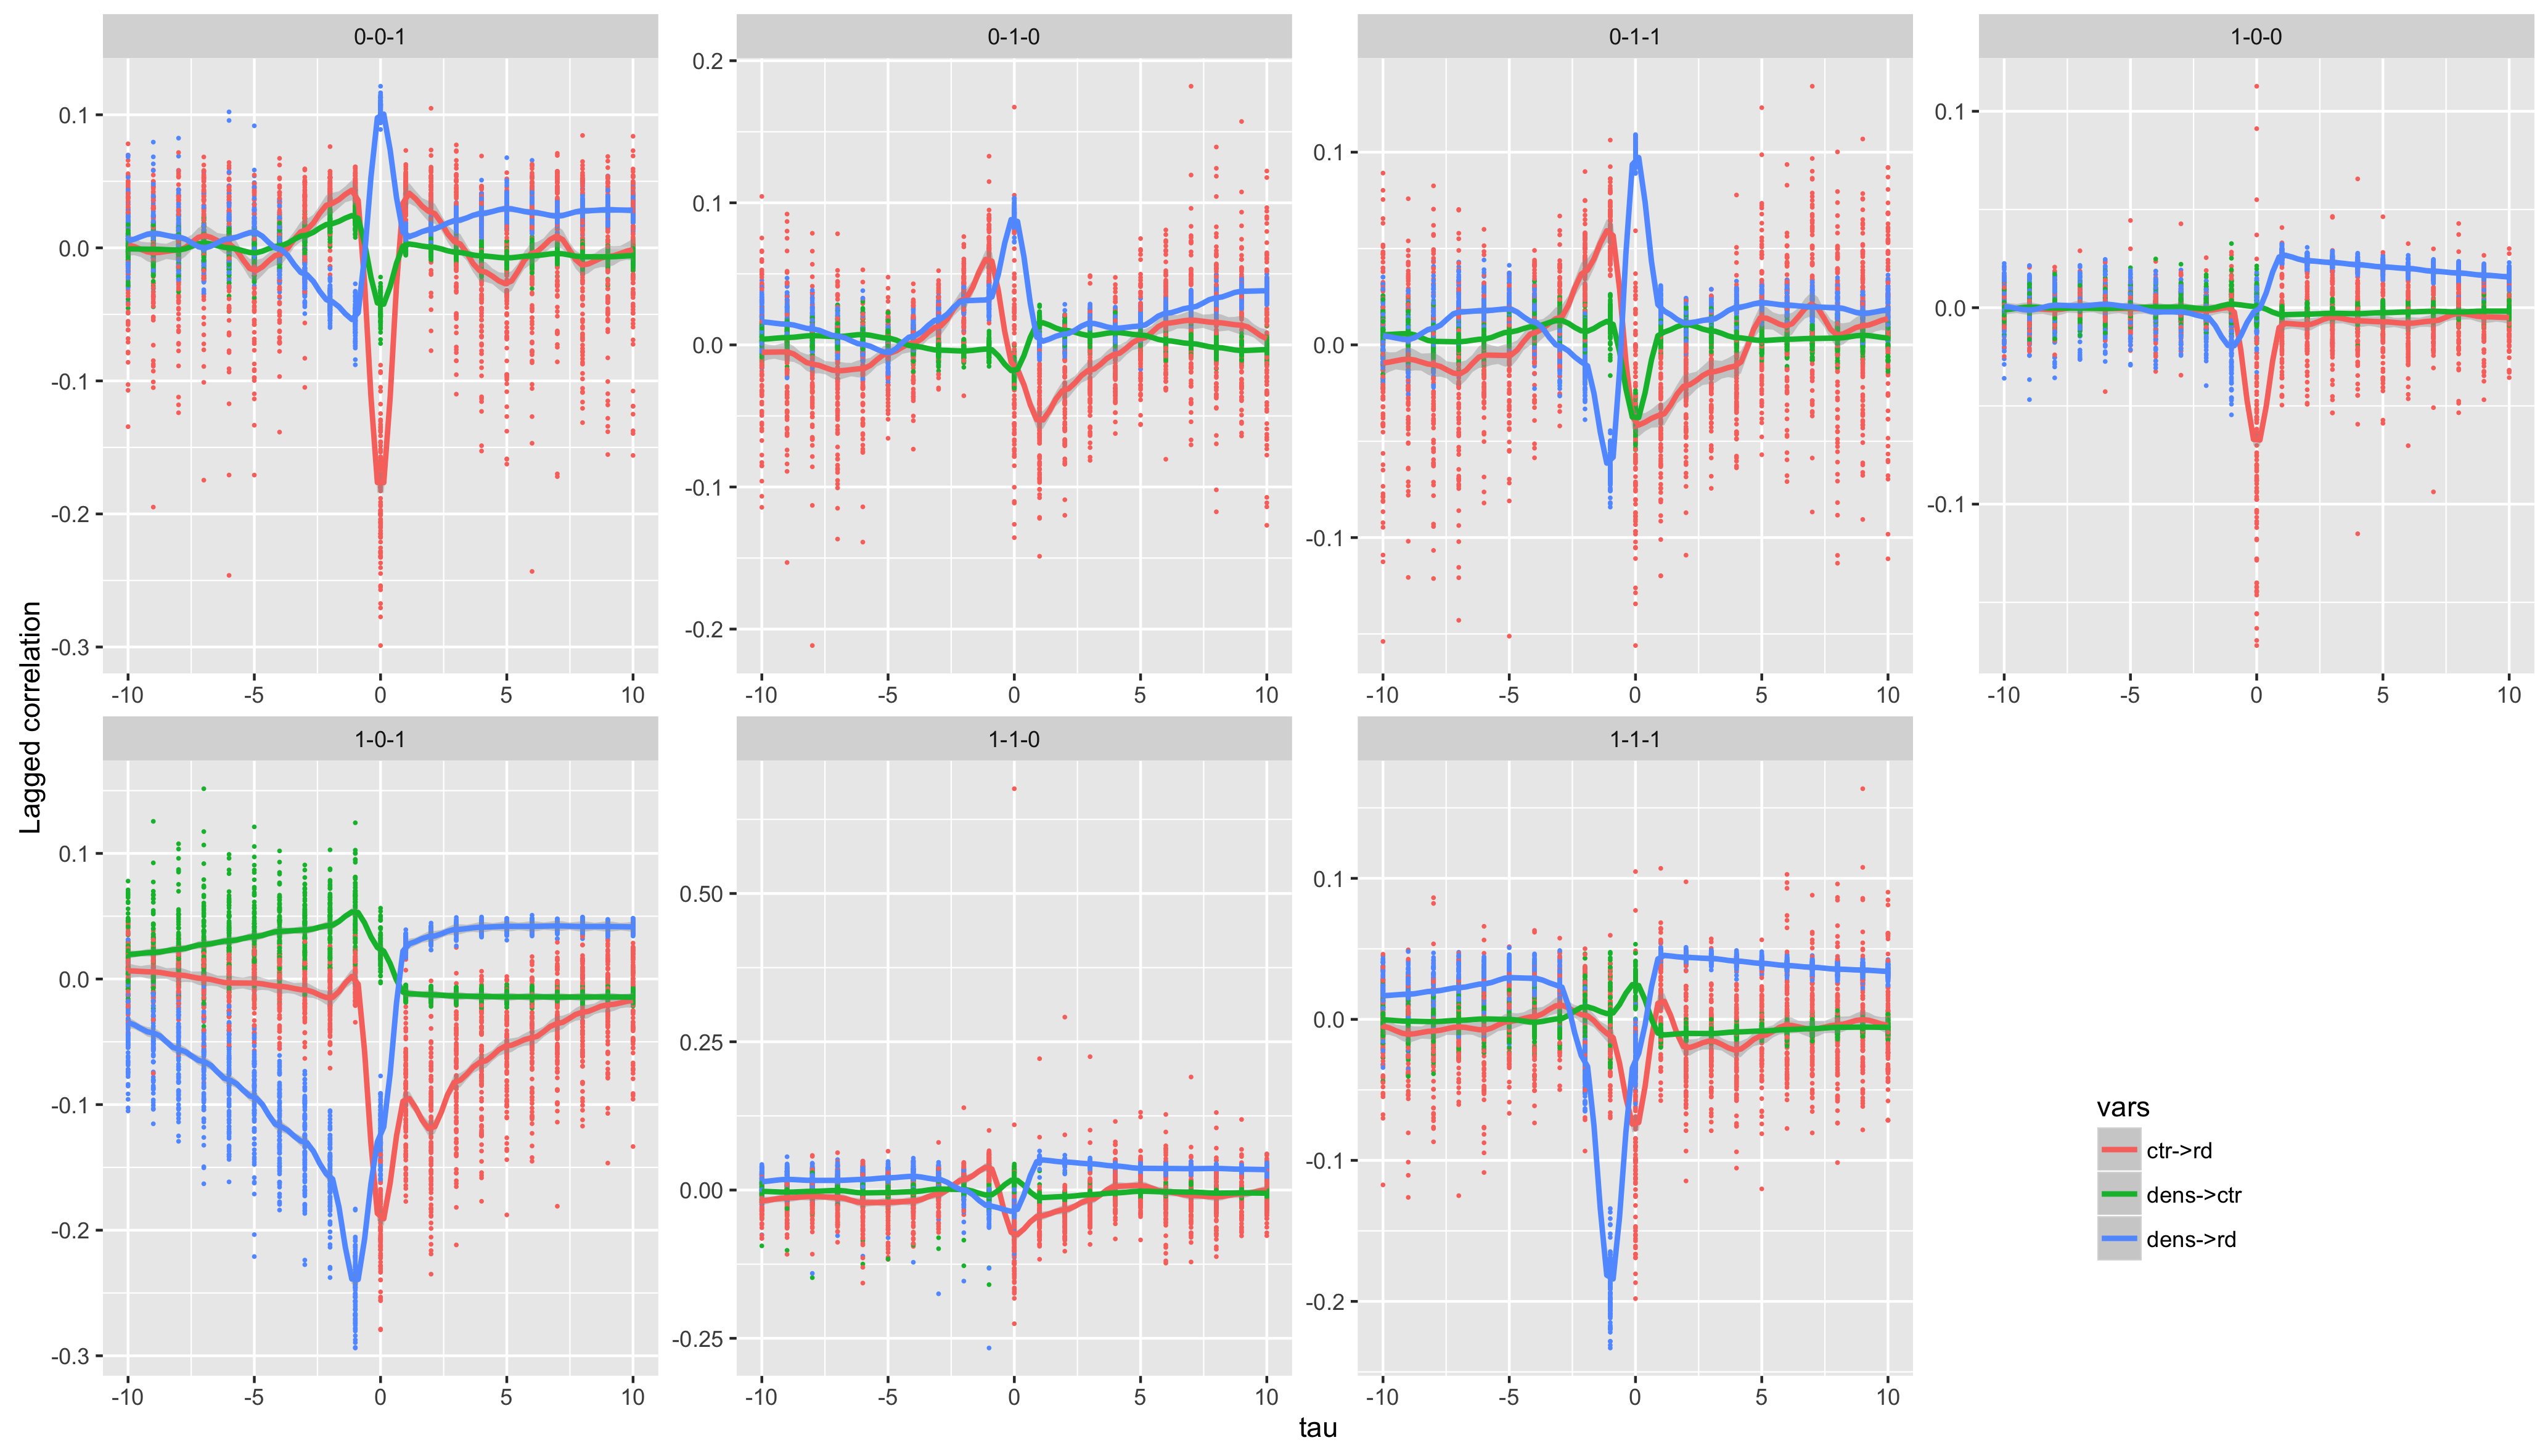
\includegraphics[width=12cm]{figures/laggedcorrs_facetextreme}
\caption{\textbf{Correlations dans le modèle RDB} (Première ligne) Exemples de configurations finales, obtenues avec $(w_{d},w_{c},w_{r})$ valant respectivement $(0,1,1)$,$(1,0,1)$, et $(1,1,1)$. (Deuxième ligne) Corrélations retardées, pour chaque combinaison des paramètres, en fonction du retard $\tau$. Les différentes couleurs correspondent }
\label{fig:exrdb}
\end{figure*}
%%%%%%%%%%%%%%%



%%%%%%%%%%%%%%%
\begin{figure*}[h]
\centering
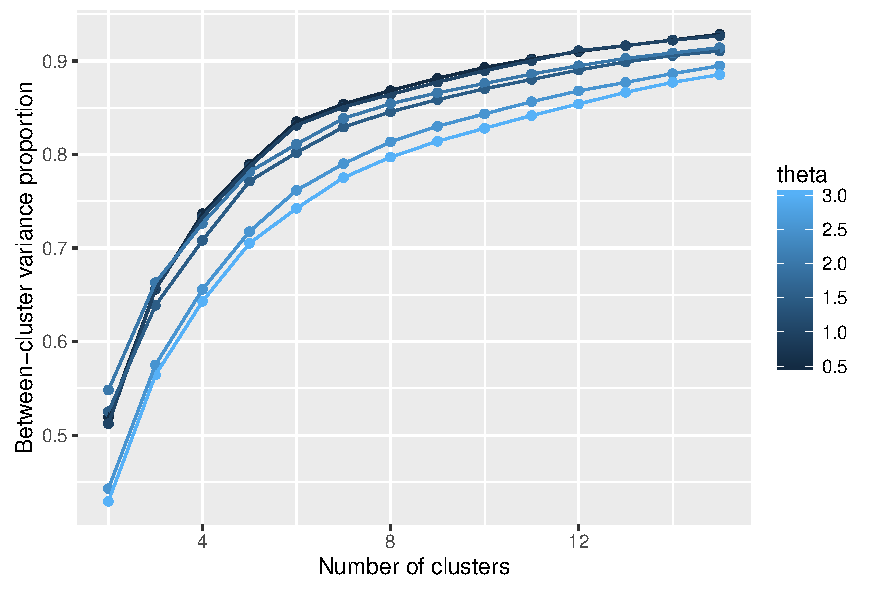
\includegraphics[width=3.9cm,height=3.2cm]{figures/ccoef-knum_valuesFALSE_theta05-3.pdf}
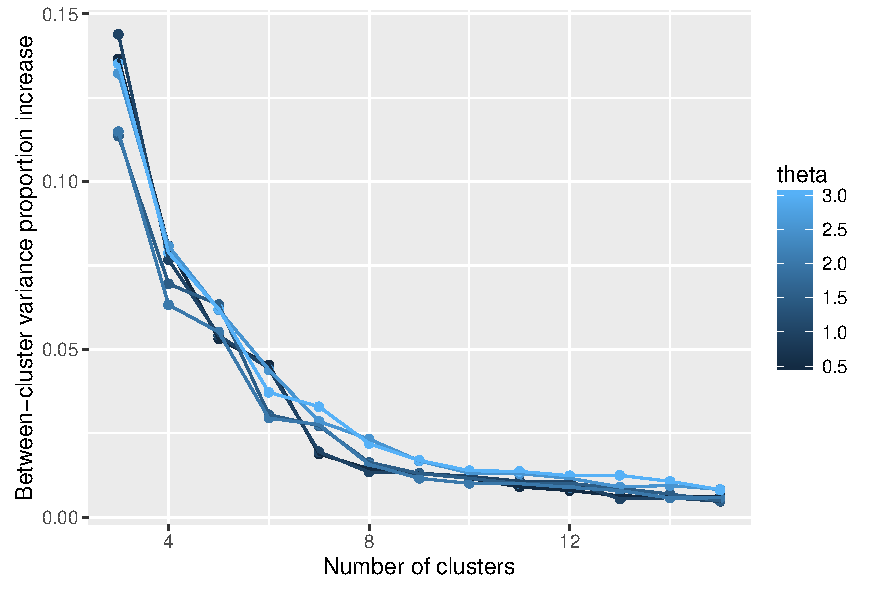
\includegraphics[width=3.9cm,height=3.2cm]{figures/dccoef-knum_valuesFALSEtheta05-3.pdf}
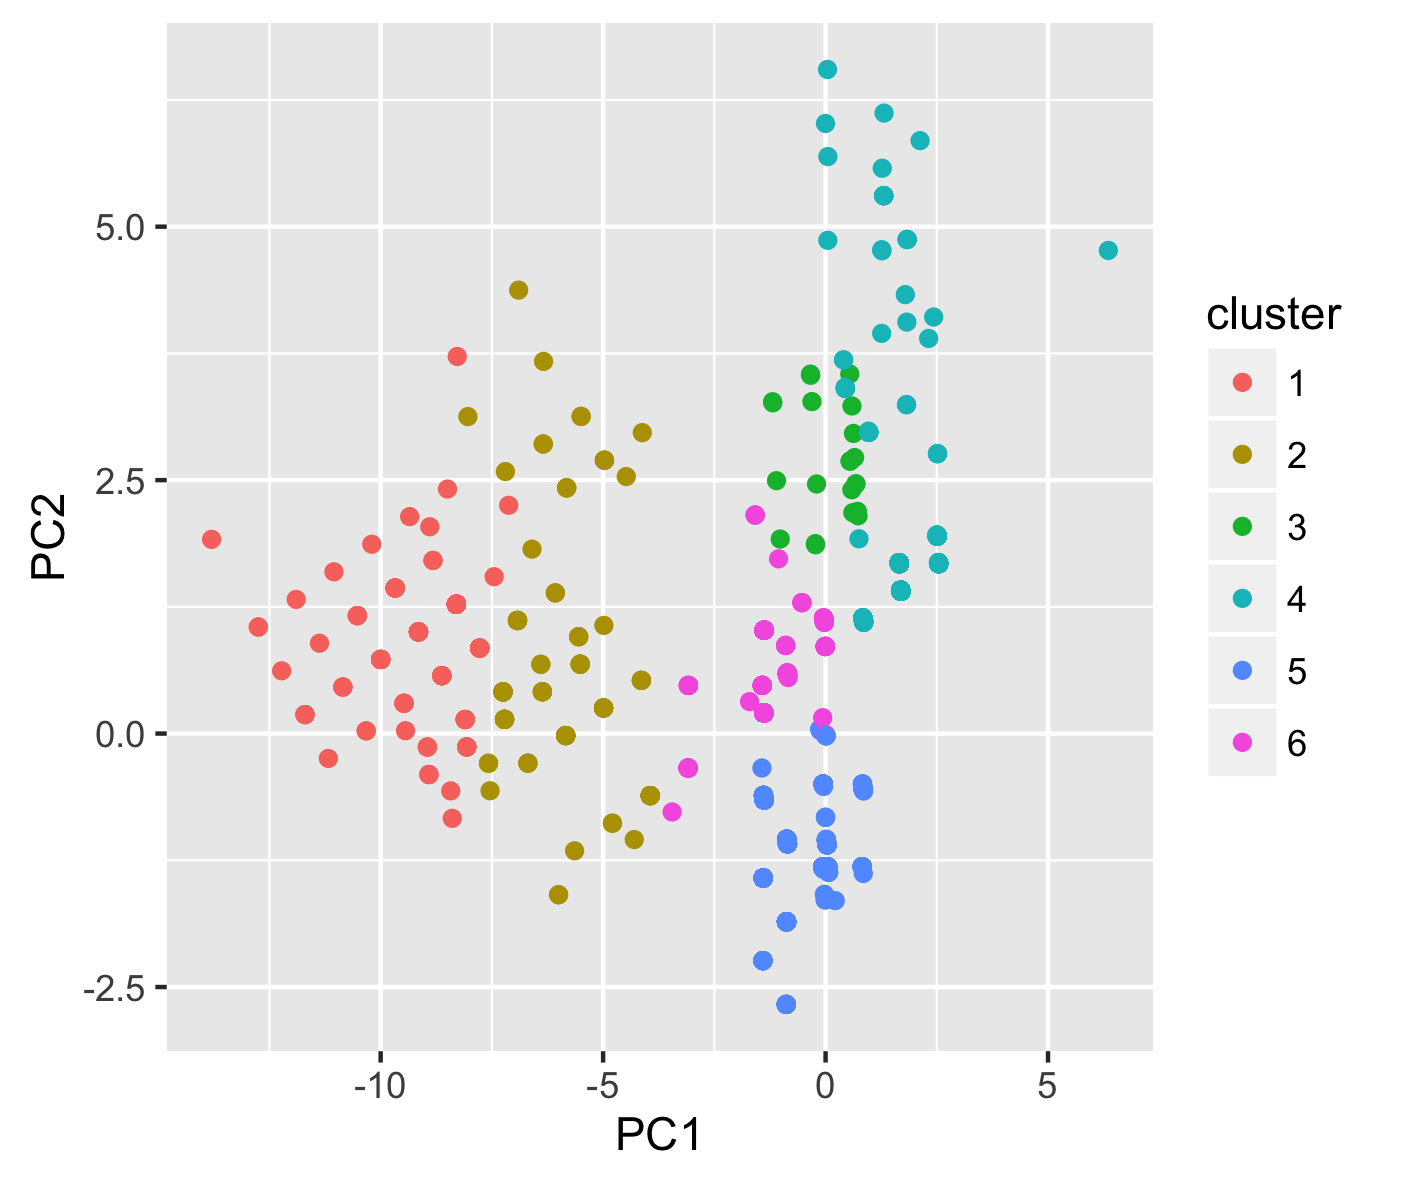
\includegraphics[width=3.9cm,height=3.2cm]{figures/clusters-PCA-features_valuesFALSEtheta2_k6}\\
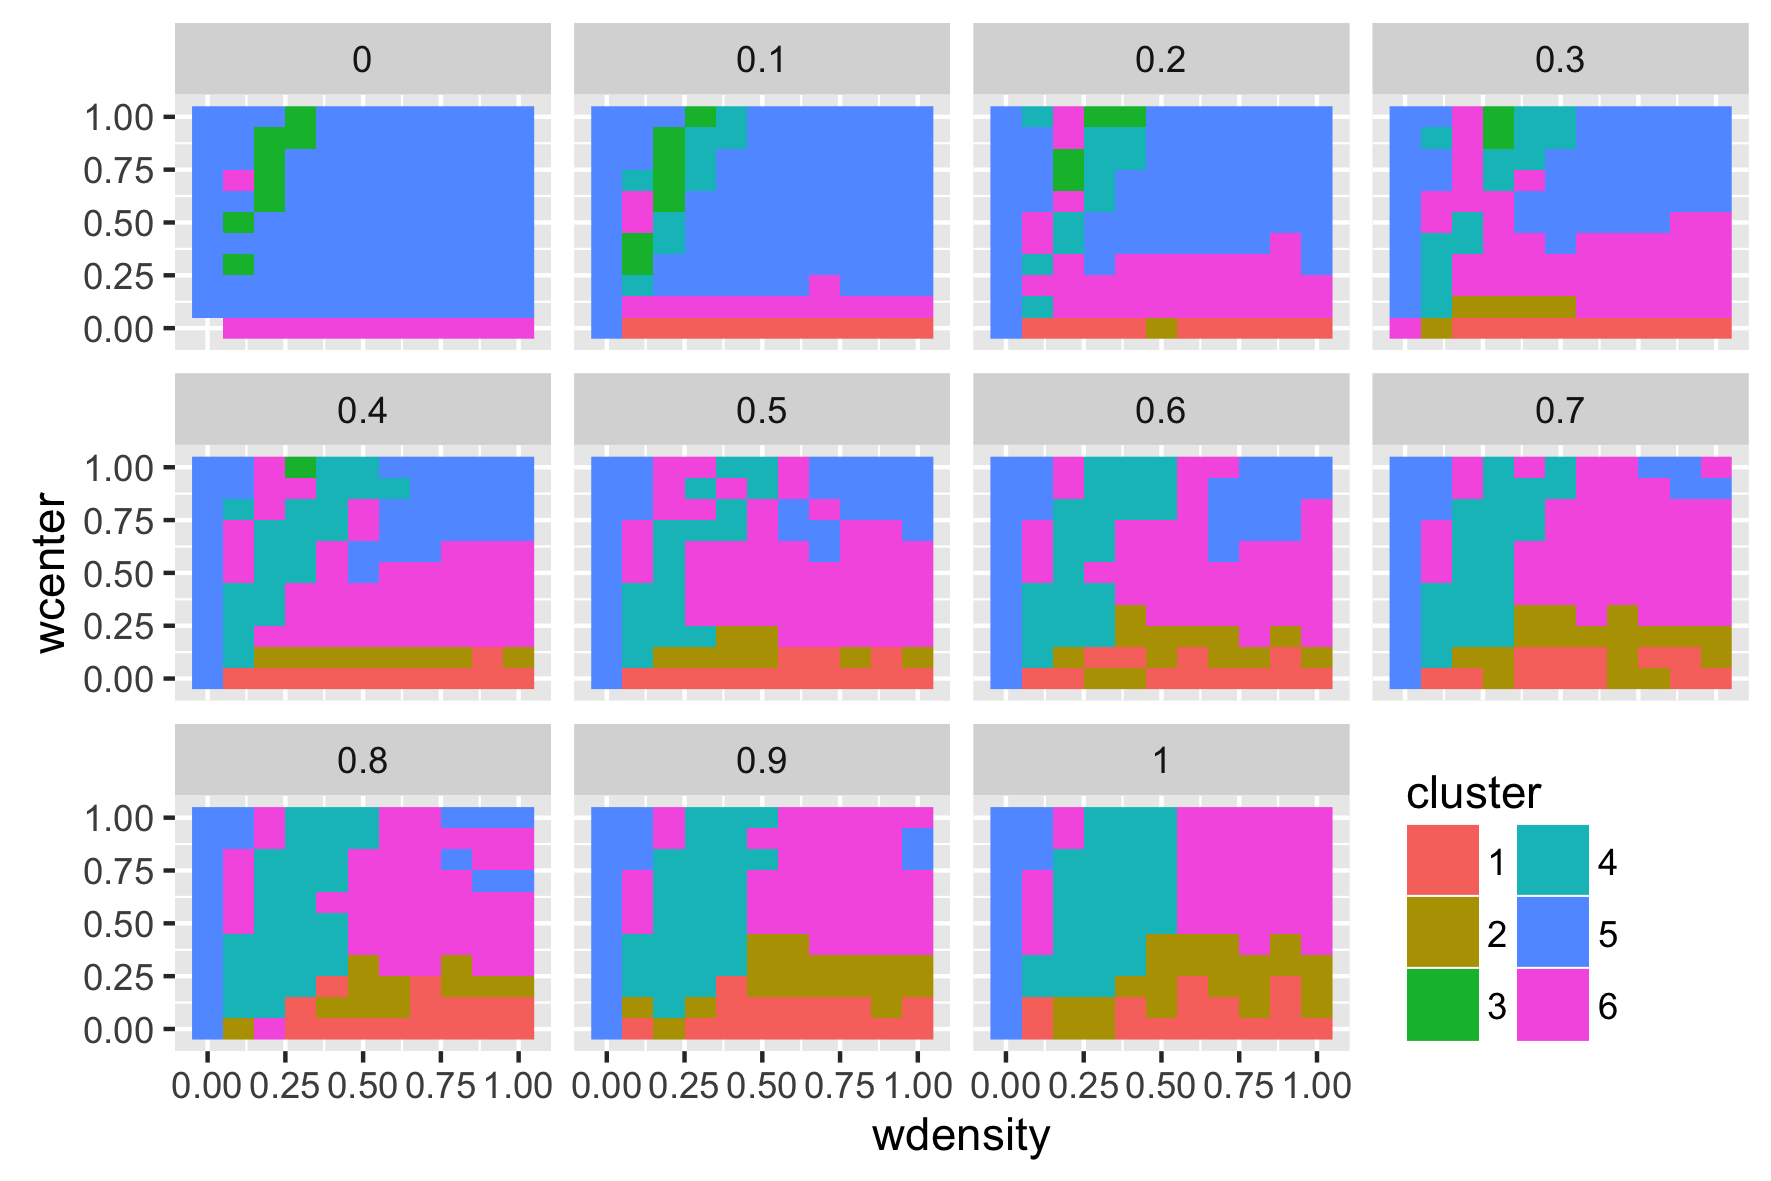
\includegraphics[width=5.9cm,height=5cm]{figures/clusters-paramfacet_valuesFALSEtheta2_k6}
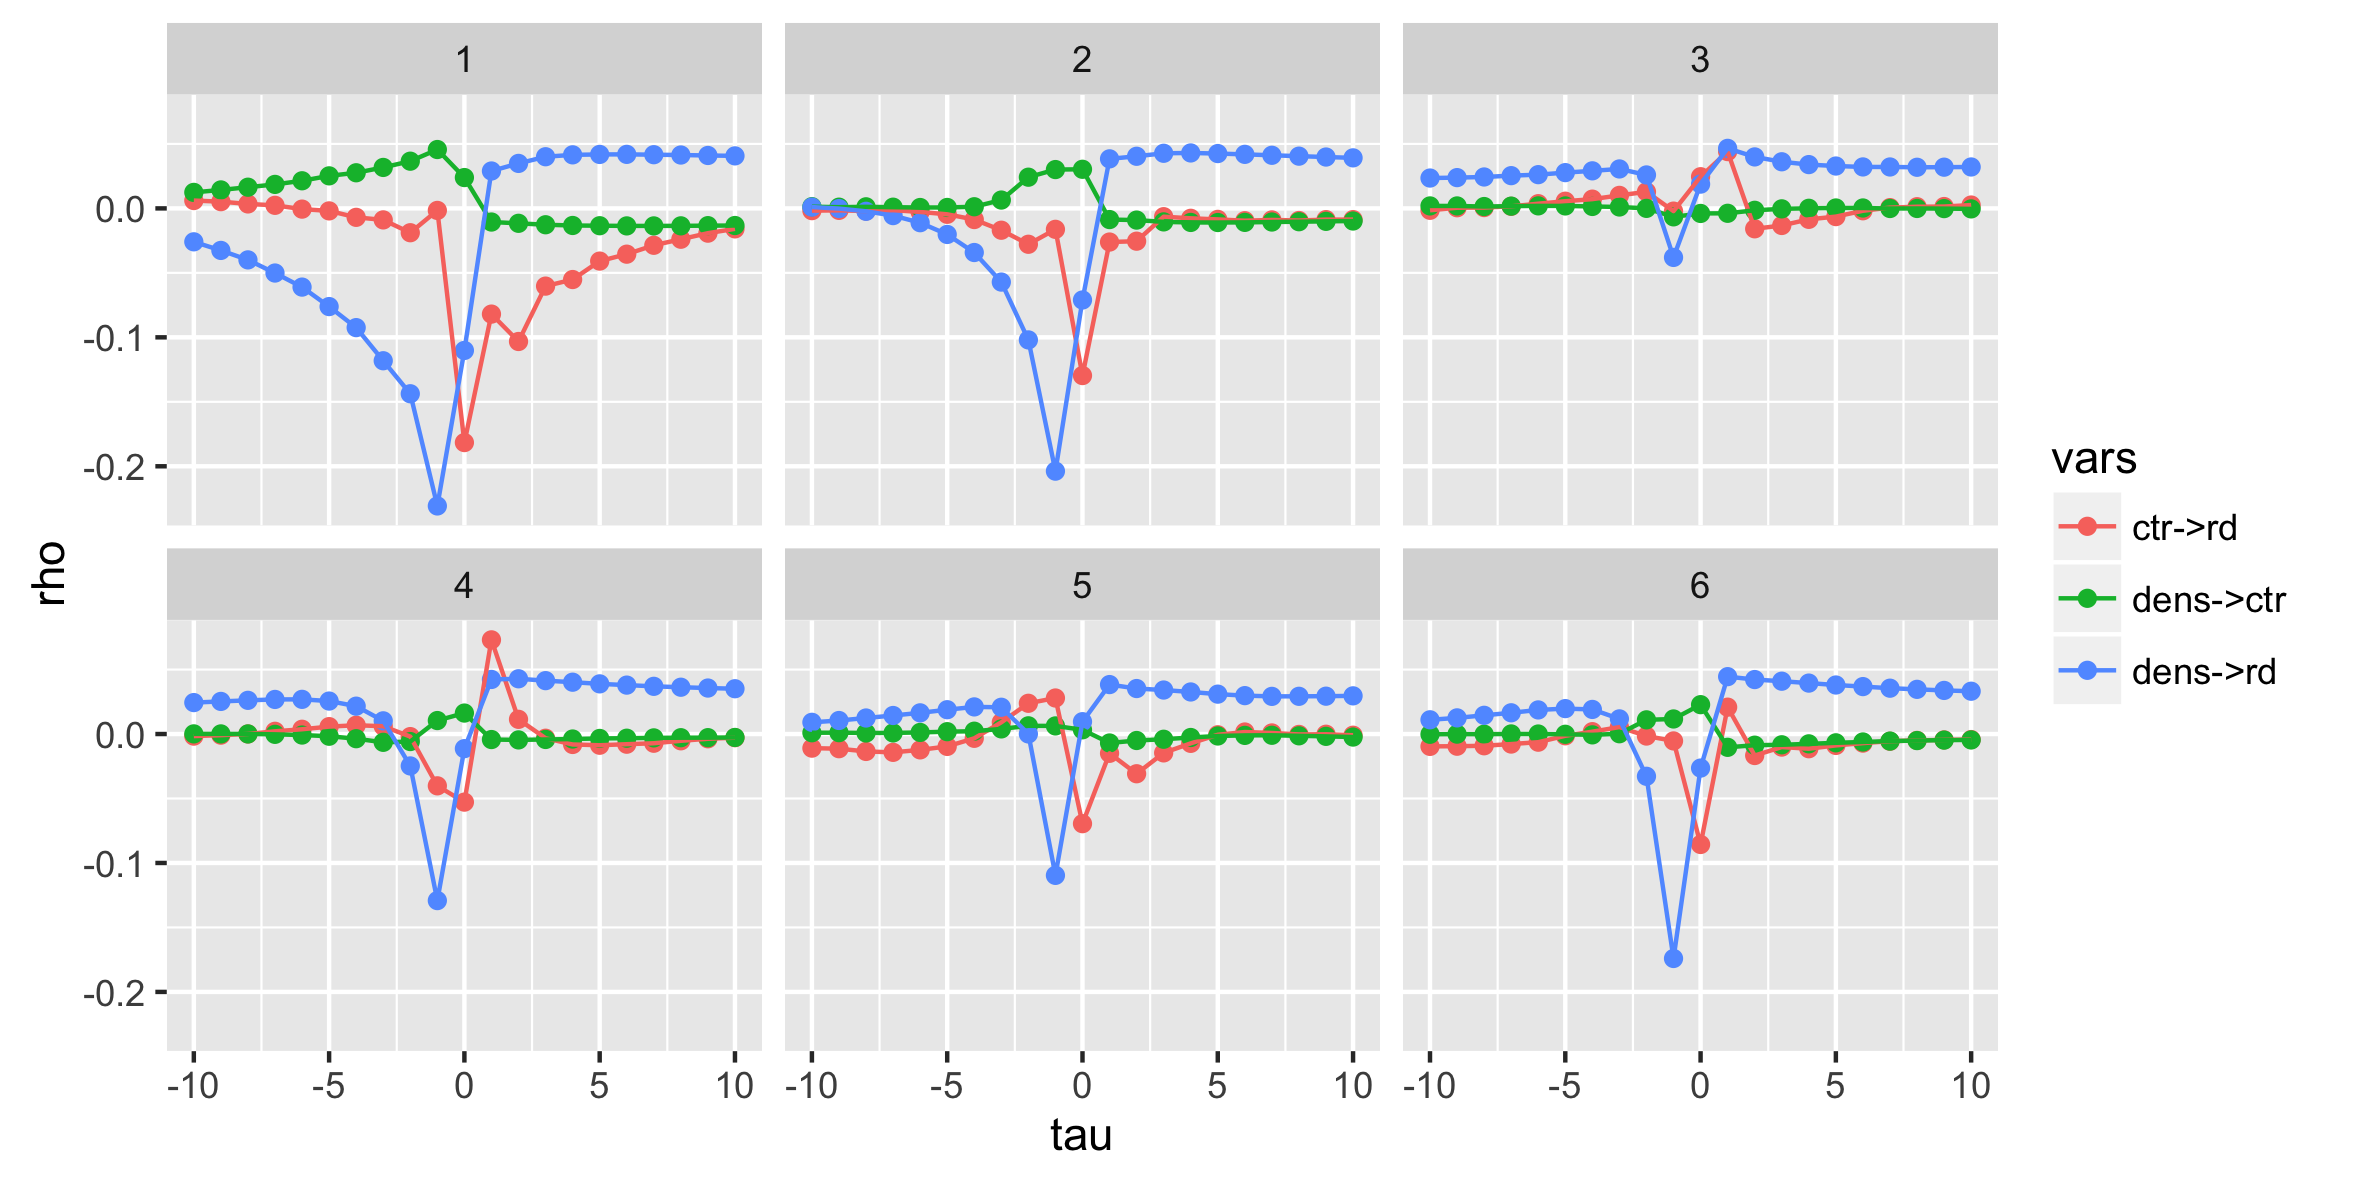
\includegraphics[width=5.9cm,height=5cm]{figures/clusters-centertrajs-facetclust_valuesFALSEtheta2_k6}
\caption{\textbf{Identification de régimes d'interactions} (Haut Gauche) Variance inter-cluster comme fonction du nombre de clusters. (Haut Milieu) Dérivée de la variance inter-cluster. (Haut Droite) Features dans un plan principal. (Bas Gauche) Diagramme de phase des régimes dans l'espace $(w_{d},w_{c},w_{r})$. (Bas Droite) Trajectoires correspondantes des centroïdes.}
\label{fig:clustering}
\end{figure*}
%%%%%%%%%%%%%%%


%%%%%%%%%%%%%%%
\subsection{Cas d'étude}


\subsubsection{Contexte}

Nous proposons une application sur un cas d'étude réel, toujours lié aux relations entre réseaux de transport et territoires.

\cite{damm1980response}

\cite{stif2007arc} projet arc express

\cite{beaucire2013grand} étude équilibrage est-ouest

\cite{sdrif2013} : SDRIF 2013

\cite{desjardins2010bataille} bataille institutionnelle état-région



%%%%%%%%%%%%%%%
\begin{figure*}[h]
\centering
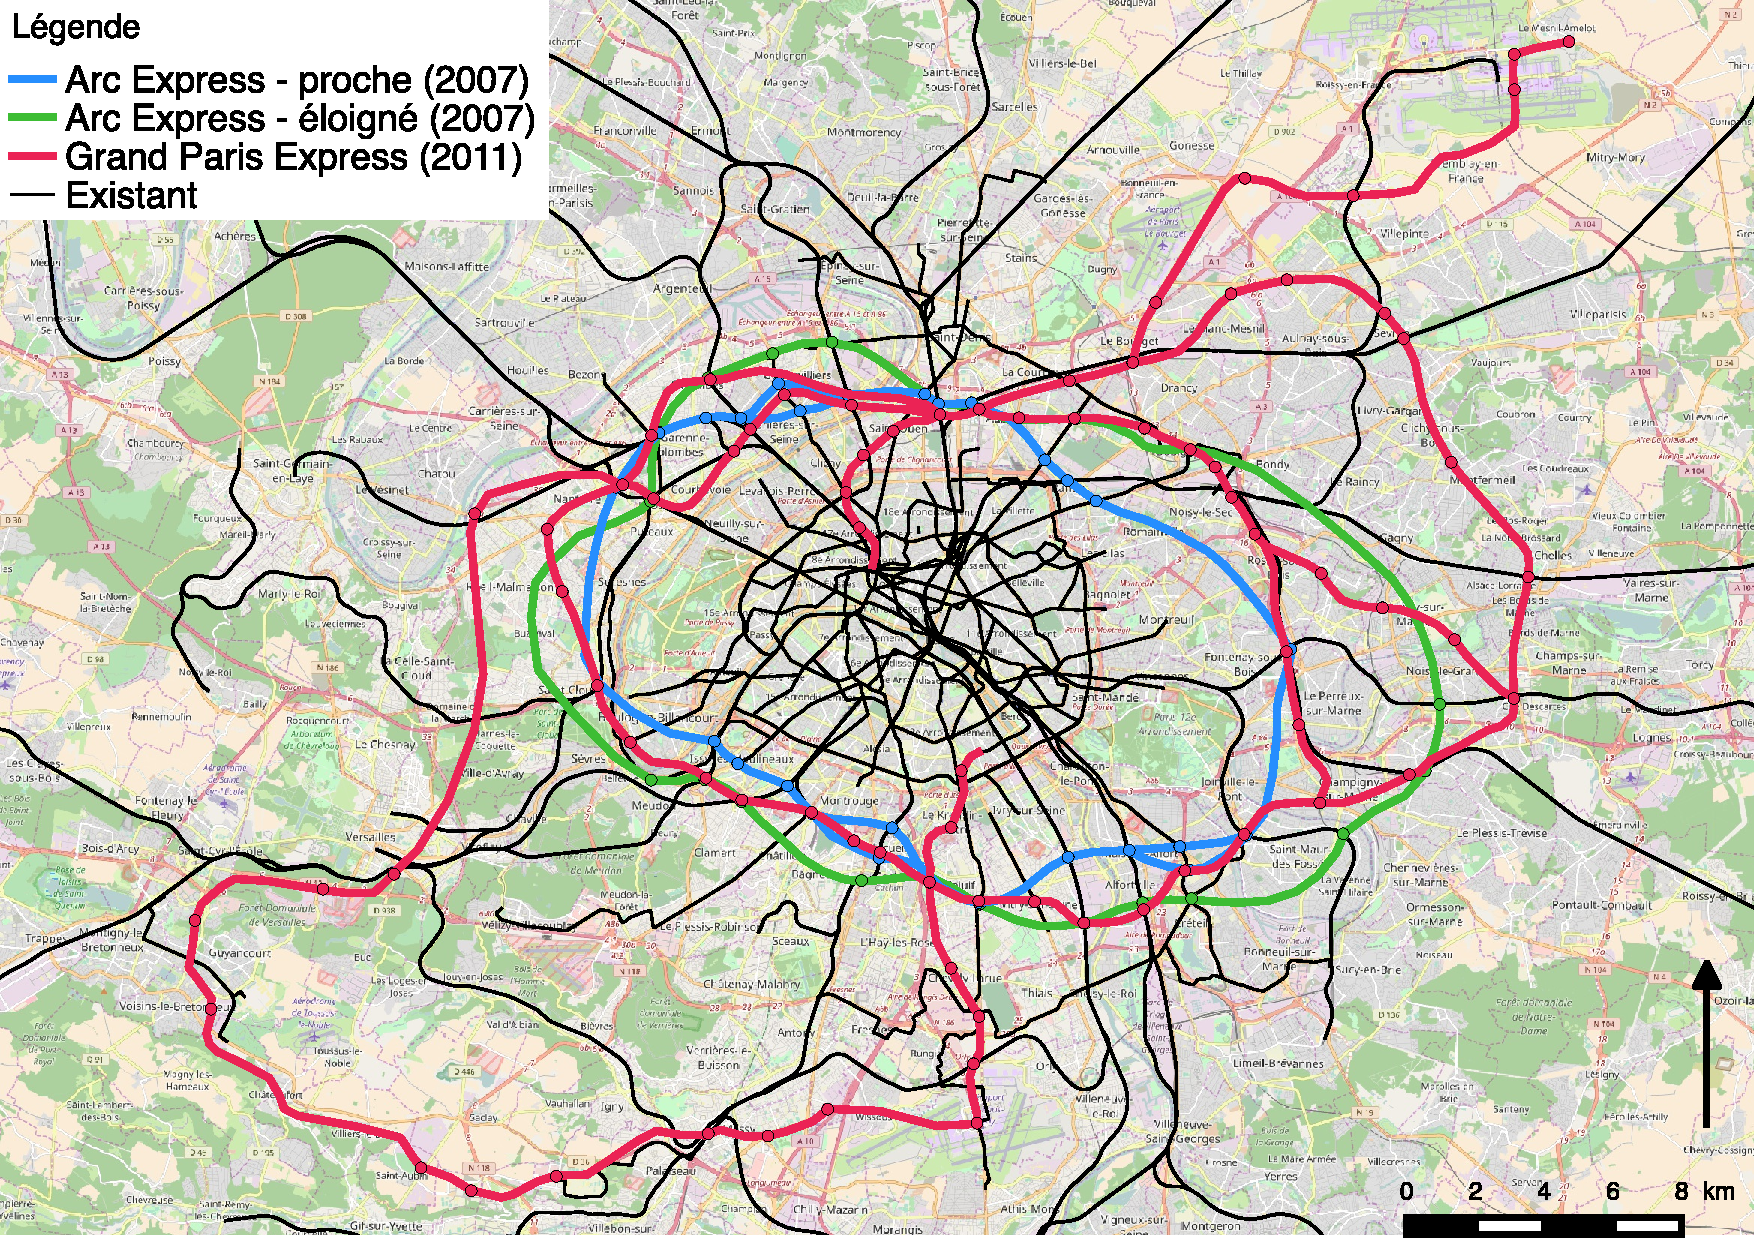
\includegraphics[width=12cm]{figures/reseaux}
\caption{\textbf{Projets de transport successifs de la métropole du Grand Paris}}
\label{fig:clustering}
\end{figure*}
%%%%%%%%%%%%%%%

\subsubsection{Données}

Le nombre de transactions après nettoyage est de 862360, se répartissant sur l'ensemble des IRIS.


\subsubsection{Résultats}

Le cas d'étude est implémenté en langage R~\cite{rcoreteam} et l'ensemble des données, du code source et des résulats sont disponibles sur un dépôt git ouvert\footnote{A l'adresse \texttt{https://github.com/JusteRaimbault/CityNetwork/tree/master/Models/SpatioTempCausality/GrandParis}. Les données de la base BIEN ne sont fournies que de manière agrégée à l'IRIS et pour les variables de prix et de crédit, pour des raisons de fermeture contractuelle de la base brute.}.






%%%%%%%%%%%%%%%
\section{Discussion}
%%%%%%%%%%%%%%%

%%%%%%%%%%%%%%%
\subsection{Diffusion}

STARMA, ondes, ergodicité etc.


%%%%%%%%%%%%%%%
\subsection{Regression Géographique Pondérée}

% lien avec GWR ?






%%%%%%%%%%%%%%%
\section{Conclusion}
%%%%%%%%%%%%%%%





%%%%%%%%%%%%%%%
%% Biblio
%%%%%%%%%%%%%%%

\bibliography{biblio,/Users/Juste/Documents/ComplexSystems/CityNetwork/Biblio/BibTeX/CityNetwork}







%%%%%%%%%%%%%%%
%% TEMPLATES
%%%%%%%%%%%%%%%

%
%
%
%\section{Section 1}
%
%\subsection{Sous-section 1}
%
%\subsubsection{Sous-sous-section 1}
%
%\begin{figure*}[h]
%   \centering  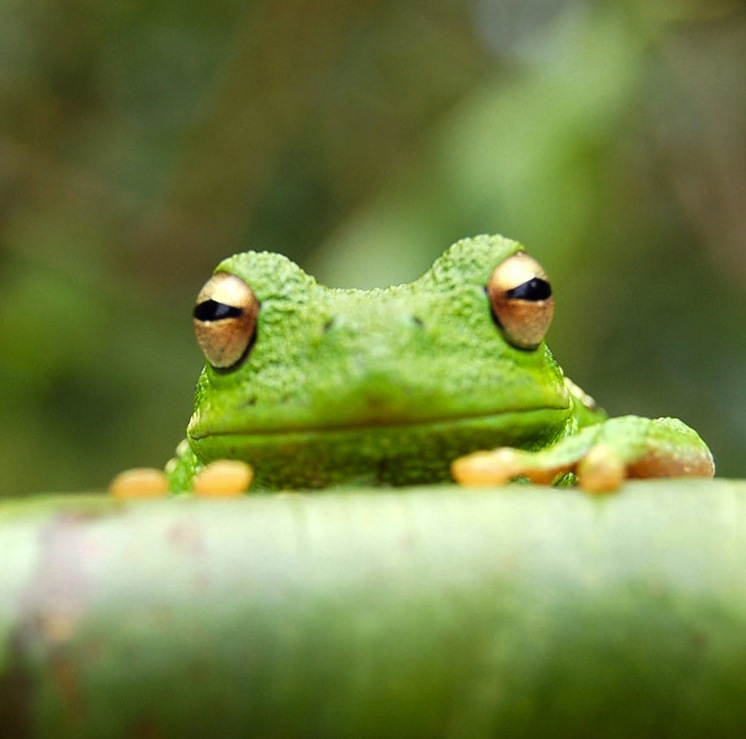
\includegraphics[width=8cm]{grenouille.jpg}
%  \caption{\label{fig:1} Une grenouille bien verte.}
%\end{figure*}
%
%\subsection{Sous-section 2}
%
%\section{Section 2}
%
%Listes :
%\begin{itemize}
%\item ligne 1 (cf. équation \ref{eq:form1})
%\item ligne 2 (cf. équation \ref{eq:form2})
%\end{itemize}
%
%Formules :
%
%\begin{equation}
%	R = \frac{d_1}{d_2}
%	\label{eq:form1}
%\end{equation}
%
%\begin{equation}
%	\sin(\alpha) = \frac{h}{l}
%    \label{eq:form2}
%\end{equation}
%
%\begin{table*}[h!]
%\begin{center}
%\caption{\label{tab:1} Exemple de tableau}
% \scriptsize
%      \begin{tabular}{|c|c|c|c|c|}
%   \hline
%   \multirow{2}*{ Clients} & \multicolumn{2}{| c |}{Départ }  & \multicolumn{2}{| c |}{ Arrivée}\\
%   \cline{2-5}
%      & Station  & Période de Temps & Station  & Période de Temps \\\hline
%   client 1 (c1) & 3  & 2 & 1 & 4 \\\hline
%   client 2 (c2)   &   2  & 2 & 3 & 3\\\hline
%   client 3 (c3)   &   2 & 2 & 3 & 4  \\\hline
%   client 4 (c4)   &   3 & 2 & 2 & 3  \\\hline
%   client 5 (c5)   &   3 & 2 & 2 & 4  \\\hline
%  client 6 (c6)   &   2  & 4 & 3 & 5\\\hline
%   client 7 (c7)   &   3  & 3 & 2 & 6  \\\hline
%   client 8 (c8)   &   1 & 5 & 3 & 6 \\\hline
%   client 9 (c9) & 2  & 6 & 3 & 7 \\\hline
%    client 10 (c10)  &   3 & 7 & 1 & 9 \\\hline
%   client 11 (c11) & 1  & 6 & 2 & 7 \\\hline
%%\hline
%\end{tabular}
%\end{center}
%\end{table*}
%
%Exemple d'algorithme :
%
%\begin{algorithm}[h!]
%\label {algo}
% \KwData{
% $G(V,A,C,R,U)$ \; \tcc{commentaire}}
% \KwResult{
% $Paths_{Cars}, \; Relocation,\; SatisfiedDemands, Paths_{Agents}  $
% }
% initialization\;
% $Paths_{Agents} \gets \emptyset $ /* l'ensemble de chemins... */ \;
% $j \gets 1$ \;
% $costPath_j  \gets 0$ \;
% \While { $ (j \le  nb_{Veh}) \wedge (costPath_j \leq 0)  $ }
% {
% $ path_j \gets Dijkstra(G(V,A, C,R)) $ \;
%$ costPath_j \gets  Cost (path_j)$ \;
%  \ForAll { $(v^{k}_{t'},v^{i}_{t}) \in path   $}
%{
% \ForAll {$ U_{r^{i}_{t'',t''+1}} $  }
% {....
% }
%$ Paths_{Cars} \gets Paths_{Cars} \cup path_j $  \;
% }
%$j \gets j+1$ \;
% }
%$Paths_{Agents} \gets  routeAgents (Relocation ); $
% \caption{un algorithme très glouton}
%\end{algorithm}
%









\end{document}